\section{Evaluation}
\label{sec:prose:evaluation}
Our evaluation of PROSE aims to answer two classes of questions: its \emph{applicability} and its \emph{performance}.
Applicability questions concern (a) our generalization of prior work in PBE
in terms of inductive specifications and witness functions; (b) generality of our library of witness functions;
(c) engineering usability of PROSE.
Performance questions concern the running time of synthesizers generated by PROSE, and the comparison of
PROSE to general-purpose non-inductive synthesizers, such as SyGuS~\cite{sygus}.

\subsection{Case Studies}
\label{sec:prose:evaluation:casestudies}
\Cref{tbl:prose:casestudies} summarizes our case studies: the prior works in inductive synthesis over numerous different
applications that we studied for evaluation of PROSE.
Of the \ref*{case:total} inductive synthesis tools we studied, \ref*{case:totaldc} can be cast as a special case of the
deductive search algorithm
methodology, which we verified by manually formulating corresponding witness functions for their algorithms.
In the other \pgfmathparse{int(\getrefnumber{case:total}-\getrefnumber{case:totaldc})}\pgfmathresult~tools, the
application domain is inductive synthesis, and our problem definition covers their application, but the original
technique is not an instance of deductive search: namely, it is enumerative
search~\cite{transit:protocols,magichaskeller} or constraint solving~\cite{quicksilver}.

\begin{table}[p!]
    \centering
    \small
    \newcounter{casenum}
    \setcounter{casenum}{-1}
    \begin{tabular}{>{\refstepcounter{casenum}}llcccc}
        \toprule
        \textbf{Project} & \textbf{Domain} & \textbf{Ded.} & \textbf{Impl.} & $\bm{\constraint}$ & $\bm{\spec'}$ \\
        \midrule
        \citet{flashfill} & String transformation & \yesmark & \yesmark & = & = \\
        \citet{flashextract} & Text extraction &  &  & $\sqsupset$ & $\sqsupset$ \\
        \citet{flashnormalize} & Text normalization &  &  & = & soft \\
        \citet{flashrelate} & Table normalization &  &  & = & = \\
        \label{case:totalreimpl}\citet{singh2012synthesizing} & Number transformation &  &  & = & = \\
        \midrule
        \citet{vldb12:semantic} & Semantic text editing & \yesmark & \nomark & = & = \\
        \citet{harris2011spreadsheet} & Table transformation &  &  & = & = \\
        \citet{andersen:procedural} & Algebra education &  &  & trace & = \\
        \citet{lau:smartedit} & Editor scripting &  &  & trace & = \\
        \citet{pldi15:swarat} & ADT transformation &  &  & = & = \\
        \citet{pldi15:osera} & ADT transformation &  &  & = & = \\
        \label{case:totaldc}\citet{miller:colorful} & Editor scripting &  &  & = & = \\
        \midrule
        \citet{transit:protocols} & Concurrent protocols & \nomark & \nomark & trace & N/A \\
        \citet{magichaskeller} & Haskell programs &  &  & = & N/A \\
        \label{case:total}\citet{quicksilver} & Relational queries &  &  & = & N/A \\
        \midrule
        \citet{raza2017automated} & Splitting of text into columns & \yesmark & \yesmark & = & = \\
        \citet{refazer} & Software refactoring & & & = & = \\
        \citet{gorinova2016end} & Reshaping of healthcare data & & & = & $\approx$ \\
        \textsf{Transformation.JSON} & Transformation of JSON trees &  &  & = & $\sqsupset$ \\
        \textsf{Extraction.JSON} & Extraction of data from JSON files &  &  & $\sqsupset$ & $\sqsupset$ \\
        \textsf{Matching.Text} & Data profiling/clustering &  &  & --- & = \\
        \label{case:totalwithnew}\textsf{Extraction.Web} & Web data extraction &  &  & $\sqsupset$ & $\sqsupset$ \\
        \bottomrule
    \end{tabular}
    \uwsinglespace
    \caption{Case studies of PROSE: prior works in inductive program synthesis.
        ``Ded.'' means ``Is it an instance of the deductive methodology?'',
        ``Impl.'' means ``Have we (re-)implemented it on top of PROSE?'', $\constraint$ is a top-level constraint kind,
        $\spec'$ lists notable intermediate constraint kinds (for the deductive techniques only).
        The bottommost section shows the new projects implemented on top of PROSE since its creation.}
    \label{tbl:prose:casestudies}
\end{table}

\begin{table}[t]
    \centering
    \begin{tabular}{lllll}
        \toprule
        \multicolumn{1}{c}{\multirow{2}{*}{\textbf{Project}}} & \multicolumn{2}{c}{\textbf{LOC}} &
            \multicolumn{2}{c}{\textbf{Development time}} \\
        \cmidrule{2-3}  \cmidrule{4-5}
        & Original & PROSE & Original & PROSE \\
        \midrule
        \citet{flashfill} & 12K & 3K & 9 months & 1 month \\
        \citet{flashextract} & 7K & 4K & 8 months & 1 month \\
        \citet{flashnormalize} & 17K & 2K & 7 months & 2 months \\
        \citet{flashrelate} & 5K & 2K & 8 months & 1 month \\
        \citet{singh2012synthesizing} & --- & 1K & --- & 2 months \\
        \midrule
        \citet{raza2017automated} & --- & 10K & --- & 2 months \\
        \citet{refazer} & & 6K & & 3 months \\
        \textsf{Transformation.JSON} & & 2K & & 1 month \\
        \textsf{Extraction.JSON} & & 3K & & 1 month \\
        \textsf{Matching.Text} & & 2K & & 3 months \\
        \textsf{Extraction.Web} & & 2.5K & & 1.5 months \\
        \bottomrule
    \end{tabular}
    \caption{Development data on the (re-)implemented projects.
        The cells marked with ``---'' either do not have an original implementation or we could not obtain historical
    data on them.}
    \label{tbl:prose:reimplementation}
\end{table}

Our industrial collaborators reimplemented \ref*{case:totalreimpl} existing systems
and created \pgfmathparse{int(\getrefnumber{case:totalwithnew}-\getrefnumber{case:total})}\pgfmathresult~new ones since
PROSE was created in \citeyear{flashmeta}.
We present data on these development efforts in \Cref{tbl:prose:reimplementation}.

\paragraph{Q1: How motivated is our generalization of inductive specification?}
Input-output examples is the most popular specification kind, observed in 12/\ref*{case:total} projects.
However, 3 projects require \emph{program traces} as their top-level specification, and 2 projects (1 prior) require
\emph{subsequences of program output}.
Boolean connectives such as $\vee$ and $\neg$ are omnipresent in subproblems across all \ref*{case:totaldc} projects
implemented using deductive search.

\paragraph{Q2: How applicable is our generic operator library?}
Most common operators across our case studies are string processing functions, due to the most popular domain being data
manipulation (11/\ref*{case:totalwithnew} projects).
Almost all projects include some version of learning conditional operators (equivalent to that of FlashFill).
List processing operators (e.g. $\mathsf{Map}$, $\mathsf{Filter}$) appear in 9/\ref*{case:totalwithnew} projects, often
without explicit realization by the original authors (for example, the awkwardly defined \textsf{Loop} operator in
FlashFill is actually a combination of \textsf{Concatenate} and \textsf{Map}).
\citet{pldi15:swarat} define an extensive library of synthesis strategies for list-processing operators in the
$\lambda^2$ project.
These synthesis strategies are isomorphic to FlashExtract witness functions; both approaches can be cast as instances of
deductive search (see \Cref{ch:related} for detailed comparison).

\paragraph{Q3: How usable is PROSE?}
\Cref{tbl:prose:reimplementation} presents some development stats on the projects that were reimplemented.
In all cases, PROSE-based implementations were shorter, cleaner, more stable and extensible.
The reason is that with PROSE, our collaborators did not concern themselves with tricky details of synthesis
algorithms, since they were implemented once and for all, as in \Cref{sec:prose:algorithm}.
Instead, they focused only on domain-specific witness functions, for which design, implementation, and maintenance are
much easier.
Notably, in case of the FlashRelate~\cite{flashrelate} reimplementation and \textsf{Extraction.Web}, our collaborators
did not have any experience in program synthesis.

The development time in \Cref{tbl:prose:reimplementation} includes the time required for an implementation to mature
(i.e. cover the required use cases), which required multiple experiments with DSLs.
With PROSE, various improvements over DSLs were possible on a daily basis.
PROSE also allowed our collaborators to discover optimizations not present in the original implementations.
We share some anecdotes of PROSE simplifying synthesizer development below.

\begin{scenario}
    One of the main algorithmic insights of FlashFill is synthesis of $\mathsf{Concat}(e_1, \dots, e_k)$ expressions
    using \emph{DAG program sharing}.
    A DAG over the positions in the output string $s$ is maintained, each edge $s[i:j]$ annotated with a
    set of programs that output this substring on a given state $\state$.
    Most of the formalism in the paper and code in their implementation is spent on describing and performing operations
    on such a DAG.
    In PROSE, the same grammar symbol is instead defined through a recursive binary operator: $f \coloneq e \,|\,
    \mathsf{Concat}(e, f)$.
    The witness function for $e$ in \textsf{Concat} constructs $\spec'$ as a disjunction of all prefixes of
    the output string in $\spec$.
    The property for $f$ is conditional on $e$ and simply selects the suffix of the output string after the given prefix
    $\semantics{e}{\state}$.
    Since PROSE caches the results of learning calls $\langle f, \spec \rangle$ for same $\spec$s, the tree of
    recursive $\mathsf{Learn}(f, \spec)$ calls becomes a DAG, as shown in \Cref{fig:prose:evaluation:dag}.
    This is \emph{the same DAG} as in FlashFill -- but with PROSE, it arises implicitly and at no cost.
    Moreover, it becomes obvious now that DAG sharing happens for any foldable operator, e.g. \textsf{ITE}, $\wedge$,
    $\vee$, sequential statements.
    \label{sc:dag}
\end{scenario}

\begin{figure}
    \newcommand{\sproblem}[2]{\ensuremath{\langle #1,\, \stringliteral{#2}\rangle}}
    \newcommand{\sproblemDisj}[3]{\ensuremath{\langle #1,\, \stringliteral{#2} \vee \stringliteral{#3}\rangle}}
    \centering
    \begin{tikzpicture}[f/.style={draw, rounded corners, inner sep=7pt, fill=PowderBlue},
                        e/.style={draw, sharp corners, shape=rectangle, inner sep=7pt, fill=LightGoldenrodYellow,
                                     minimum width=2.2cm},
                        concat/.style={},
                        every path/.style={-Stealth, rounded corners=10pt}]
        \node[f] (t202) {\sproblem{f}{202}};
        \node[concat, anchor=west, below=0.5cm of t202.south east] (conc202) {\textsf{Concat}};
        \draw (t202.west) |- (conc202);
        \node[f, anchor=west] at ($(conc202.south) + (1cm, -2cm)$) (t02) {\sproblem{f}{02}};
        \draw (conc202.south) |- (t02);
        \node[concat, anchor=west, below=0.5cm of t02.south east] (conc02) {\textsf{Concat}};
        \draw (t02.west) |- (conc02);
        \node[f, below right=0.5cm of conc02] (t2) {\sproblem{f}{2}};
        \draw (conc02.south) |- ($(t2.north west)!0.33!(t2.south west)$);
        \draw ($(conc202.south west)!0.5!(conc202.south)$) |- ($(t2.south west)!0.33!(t2.north west)$);

        \node[e, right=11.5cm of t202] (a202) {\sproblem{e}{202}};
        \node[e, below=0.25cm of a202] (a20) {\sproblem{e}{20}};
        \node[e, below=0.25cm of a20] (a2) {\sproblem{e}{2}};
        \node[e, below=0.25cm of a2] (a02) {\sproblem{e}{02}};
        \node[e, below=0.25cm of a02] (a0) {\sproblem{e}{0}};

        \draw[dashed] (t202) -> (a202);
        \node[e, right=4.5cm of conc202] (adisj) {\sproblemDisj{e}{2}{20}};
        \draw[dashed] (conc202) -> (adisj);
        \draw[dashed] (adisj) -> (a20);
        \draw[dashed] (adisj) |- ($(a2.north west)!0.33!(a2.south west)$);
        \draw[dashed] (t02) -> (a02);
        \draw[dashed] (conc02) -> (a0);
        \coordinate (target) at ($(a2.south west)!0.33!(a2.north west)$);
        \coordinate (cut) at (adisj.east|-target);
        \draw[dashed] (t2.east) -| (cut) -> (target);
    \end{tikzpicture}
    \caption{A DAG of recursive calls that arises during the deductive search process for a recursive binary operator
        $f \coloneq e \;|\; \mathsf{Concat}(e,\, f)$.
        As described in \Cref{sc:dag}, it is isomorphic to an explicitly maintained DAG of substring programs in the
        original FlashFill implementation~\cite{flashfill}.}
    \label{fig:prose:evaluation:dag}
\end{figure}

\begin{scenario}
    During reimplementation of FlashFill, a new operator was added to its substring extraction logic: \emph{relative
    positioning},
    which defines the right boundary of a substring depending on the value of its left boundary.
    For example, it enables extracting substrings as in ``ten characters after the first digit''.
    This extension simply involved adding three \texttt{let} rules in the DSL, which (a) define the left boundary
    position using existing operators; (b) cut the suffix starting from that position; (c) define the right boundary in
    the suffix.
    While such an extension in the original FlashFill implementation would consume a couple of weeks, in PROSE it
    took only a few minutes.
\end{scenario}

\begin{scenario}
    A CSS selector is a function $\mathsf{Document} \to \mathsf{Set}\langle \mathsf{DOMNode}\rangle$.
    It is a path specification for a DOM node where each element in the path is a predicate on the corresponding
    ancestor (i.e.  the ancestor's tag or its class), and each edge in the path descends to all children of the
    preceding element that satisfy a certain property~\cite{css3selectors}.

    A spec synthesis of CSS selectors is a subset of selected DOM nodes.
    Using an enumerative search for this problem induces an exponential blowup: it starts with an input state (an HTML
    document) and iteratively constructs all possible CSS selectors.
    Since they may select arbitrary subsets of the DOM tree, the resulting search is infeasible.

    In contrast, a deductive approach starts with an \emph{output} (a set of nodes), and deduces examples for the
    intermediate subexpressions (prefixes of the desired CSS selector).
    This process follows the DOM tree \emph{upwards}, instead of \emph{downwards}, and therefore is by construction
    finite.
    Moreover, the number of deduction steps is bounded by the tree depth.
\end{scenario}

\begin{figure}[p!]
    \centering
    \begin{tikzpicture}
        \node[anchor=south west, inner sep=0] (img) at (0,0) {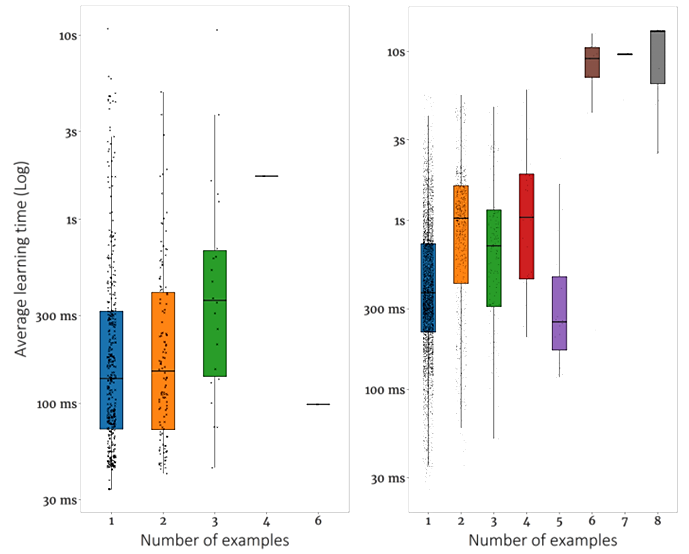
\includegraphics[width=\textwidth]{figures/perf}};
        \begin{scope}[x={(img.south east)}, y={(img.north west)}]
            \node[inner sep=10pt, rounded corners, fill=Tan] at (0.3, 1) {FlashFill};
            \node[inner sep=10pt, rounded corners, fill=Tan] at (0.78, 1) {FlashExtract};
            \node[fill=white] at (0.3, 0.02) { Number of examples };
            \node[fill=white] at (0.78, 0.02) { Number of examples };
            \node[fill=white, rotate=90] at (0.03, 0.52) { Average learning time (Log) };
        \end{scope}
    \end{tikzpicture}
    \caption{Performance evaluation of the reimplementations of FlashFill~\cite{flashfill} and
    FlashExtract~\cite{flashextract} on top of the PROSE framework.
    Each dot shows average learning time per iteration on a given scenario.
    The scenarios are clustered by the number of examples (iterations) required to complete the task.
    \emph{Left:} 531 FlashFill scenarios.
    \emph{Right:} 6464 FlashExtract scenarios.}
    \label{fig:prose:evaluation:perf}
\end{figure}

\subsection{Experiments}
\label{sec:prose:evaluation:experiments}

\paragraph{Performance \& Number of examples}
\Cref{fig:prose:evaluation:perf} shows performance and the number of examples of our FlashFill and FlashExtract
reimplementations on top of the PROSE framework.
The overall performance is comparable to that of the original system, even though the implementations differ
drastically.
For example, the runtime of the original implementation of FlashExtract varies from 0.1 to 4 sec, with a median of 0.3
sec~\cite{flashextract}.
The new implementation (despite being more expressive and built on a general framework) has a runtime of
$0.5-3$x the original implementation, with a median of 0.6 sec.
This performance is sufficient for the PROSE-based implementation to be successfully used in industry instead of the
original one.

\paragraph{VSA Volume}
There is no good theoretical bound on the time of VSA clustering (the most time-consuming operation in the deductive
search).
However, it is evident that the output VSA volume is proportional to the clustering time.
Thus, to evaluate it, we measured the VSA volume on our real-life benchmark suite.
As \Cref{fig:prose:evaluation:volume} shows, even for large inputs it never exceeds $8000$ nodes (thus explaining
efficient runtime), whereas VSA size (i.e. number of learned programs) may approach $10^{13}$.

\begin{figure}[t]
    \centering
    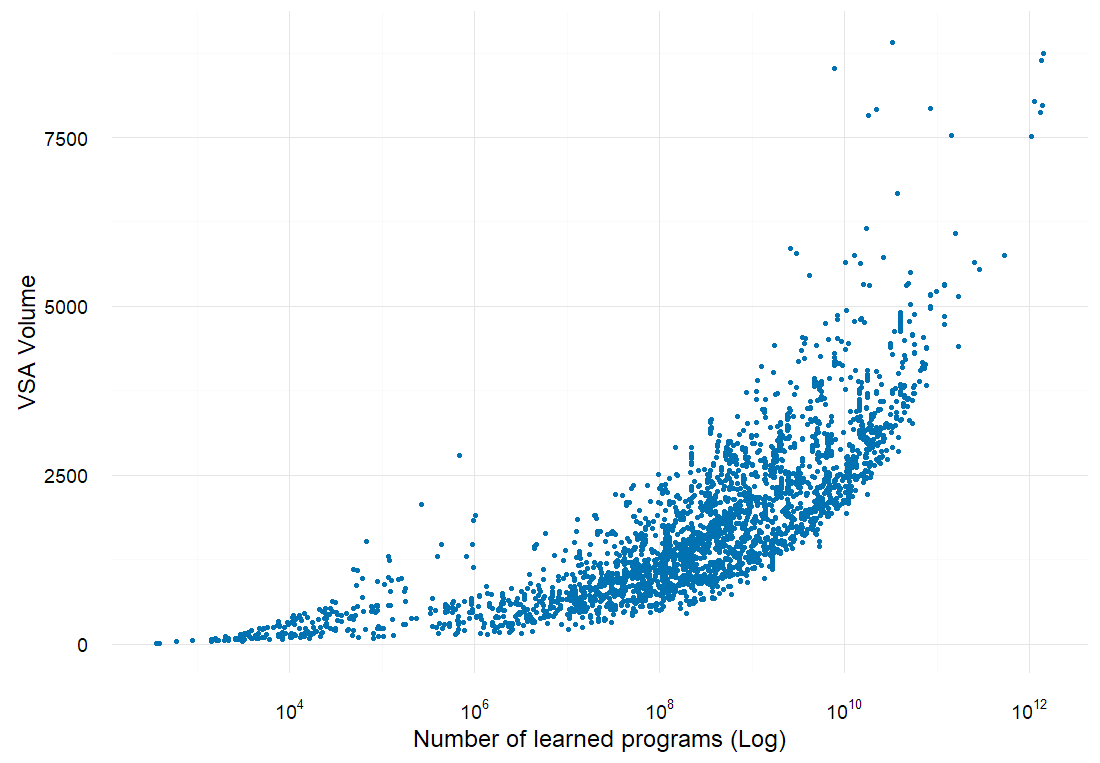
\includegraphics[width=1.0\linewidth]{figures/vsa-volume}
    \uwsinglespace
    \caption{The relationship between VSA volume and VSA size (i.e. number of programs) for the complete VSAs learned to
    solve 6464 real-life FlashExtract scenarios.}
    \label{fig:prose:evaluation:volume}
\end{figure}
